\chapter{Desenvolvimento do sistema}
\label{chap:etapas_desenvolvimento}

Nesta seção iremos apresentar detalhadamente os passos e ferramentas necessárias para elaboração da aplicação web Mercado Universitário. A medida que for sendo detalhado cada passo seguido, será apresentada sua finalidade e o motivo do uso das ferramentas ali utilizadas para produção do mesmo. \par
Intencionalmente as seções estão organizadas de forma cronológica a linha de desenvolvimento da aplicação, dessa forma fica mais fácil o entendimento e execução futura dos passos necessários para validar o atual projeto por terceiros. Foi buscado não só organizar as subseções desta seção, bem como seguir uma metodologia ágil de desenvolvimento para construção do sistema web, como será apresentado na próxima subseção.

\section{Método ágil de desenvolvimento}

Desenvolvimento Guiado a Testes(TDD - do inglês Test Driven Development) foi a metodologia ágil de desenvolvimento para produção dessa aplicação devido a vários fatores, como:
\begin{itemize}  
\item Necessidade de \textit{feedbacks} rápidos sobre as funcionalidades implementadas sistema
\item Como o código será aberto, fica mais fácil a verificação de códigos bons e sem \textit{bugs} feitos por terceiros
\item A produtividade aumenta bastante, devido a ser fácil a detecção de \textit{bugs} por meio dos testes do TDD
\item Como será um projeto que estará constantemente sendo atualizado, fica-se mais fácil a implementação de novas funcionalidades e \textit{refactoring} do observando se tal mudança afeta outras partes do sistema.
\end{itemize}
No projeto Mercado Universitário foi aplicado três tipos de testes automatizados fornecidos pelo TDD, os testes unitários, os testes de integração e testes de segurança da aplicação. Tais testes serão melhor detalhados na seção \ref{tdd}.

\section{Atores do sistema}

Para que seja possível definir melhor o escopo dos requisitos do sistema(que será apresentado na seção \ref{requisitos}), foi preciso identificar os atores que farão parte da aplicação. Dessa forma será possível determinar e entender de maneira correta as responsabilidades de cada tipo de usuário do sistema. \par
Cada ator terá seu nível de acesso definido na aplicação, que será percebido na coluna “responsabilidade” que se encontra no quadro 1. Como pode ser percebido no quadro 1, os tipos de atores podem realizar tarefas distintas como também tarefas que têm um mesmo propósito. \par
Em tal projeto, inicialmente, não será necessário a presença de um ator como administrador geral do sistema devido a se tratar de um projeto piloto em uma única universidade, sem a necessidade constante de adicionar novas universidades e cursos da mesma. Tal ponto será apresentado e discutido melhor na seção de trabalhos futuros que se encontra na seção XXX.

\begin{tabularx}{0.9\textwidth} { 
  | >{\raggedright\arraybackslash}X 
  | >{\raggedright\arraybackslash}X 
  | >{\raggedright\arraybackslash}X 
  | >{\raggedright\arraybackslash}X | }
 \hline
 Ator & Descrição & Responsabilidade & Acesso a área restrita? \\
 \hline
 Convidado  & Qualquer pessoa do âmbito universitário que deseja comprar ou vender produtos  & Cadastrar-se como novo usuário do sistema & Não  \\
\hline
Cliente & Discentes, funcionários, ou moradores da região próxima a universidade & Visualizar categorias, produtos, vendedores, \textit{reviews} e seus próprios pedidos; Cadastrar novos pedidos e \textit{reviews}; Atualizar seus próprios \textit{reviews} e dados cadastrais & Não \\
\hline
Vendedor & Discentes, funcionários, ou moradores da região próxima a universidade que obtém renda a partir do comércio informal & Visualizar clientes, seus pedidos e seus \textit{reviews}; Cadastrar novos produtos; Atualizar seus produtos e dados cadastrais & Sim \\
\hline
\end{tabularx}

\section{Levantamento de requisitos}\label{requisitos}

O levantamento de requisitos é completamente fundamental para a elaboração do desenvolvimento desse sistema, pois é nessa fase que entende-se o problema e as necessidades dos \textit{stakeholders}(Grupo de interesses) para propor as melhores soluções possíveis para resolução desse problema. Nesta seção iremos apresentar os requisitos funcionais e não funcionais do sistema.

\subsection{Requisitos funcionais}

Tais requisitos são necessários para atender as regras de negócio do sistema web, como o próprio nome já diz, são as funcionalidades do sistema.  Segundo \cite{sommerville2007engenharia}, os requisitos funcionais são as asserções de serviços que a aplicação deve proporcionar, como o sistema deve responder a entradas específicas e como o sistema deve proceder em determinadas situações. \par
Será definidas as seguintes denominações de prioridade de implementação no sistema:
\begin{itemize}  
\item \textbf{Essencial:} requisito imprescindível para o funcionamento do sistema em que o sistema. Em sua ausência, o sistema não entra no ar.
\item \textbf{Importante:} requisito em que deve ser implantado o mais rápido possível, pois sem o qual o sistema entra em funcionamento, mas de forma não satisfatória.
\item \textbf{Desejável:} requisito ao qual pode ser implantado sem pressa, pois não compromete o funcionamento do sistema, já que o mesmo funciona de forma satisfatória sem ele.
\end{itemize} \par
Não será necessário abordar todos os requisitos funcionais nesta seção, pois muitas vezes trata-se de requisitos parecidos e muitas vezes facilmente dedutíveis. Diante disso, serão apresentados apenas os principais para que tenha-se uma visão geral deles. A lista contendo todos os requisitos funcionais estará nos apêndices.

\textbf{RF02 - Fazer login} \par
\textbf{Prioridade:} Essencial \par
\textbf{Atores:} Cliente \par
\textbf{Descrição:} Após realizar o cadastro, o usuário estará apto a fazer o login na plataforma para ter acesso a todo o ambiente que o sistema proporciona. O login é totalmente essencial por ter a capacidade de identificar unicamente cada usuário do sistema por meio do seu e-mail e senha, fazendo assim com que o resto do sistema traga informações relativas em relação aquele ator que acabou de logar, como por exemplo retornar apenas compras realizadas pelo ator logado. \par
\textbf{Fluxo de eventos:} \par
\textbf{Principal} \par
\begin{enumerate}
  \item O usuário insere suas credenciais(e-mail e senha) e clica no botão para logar
  \item O sistema redireciona para a página de produtos e informa que o login foi bem sucedido.
\end{enumerate}

\textbf{Secundário}

\begin{enumerate}
  \item O usuário insere suas credenciais(e-mail e senha) e clica no botão para logar
  
  \item O sistema renderiza a mesma página e informa que o login não foi bem sucedido devido a divergência nos dados cadastrais
  
  \item O usuário corrige as credenciais no formulário e realiza uma nova submissão dos dados

\end{enumerate}

\textbf{RF08 - Cadastrar \textit{review} de um vendedor} \par
\textbf{Prioridade:} Essencial \par
\textbf{Atores:} Cliente \par
\textbf{Descrição:} O cliente poderá compartilhar sua opinião acerca de algum vendedor por meio da página de cadastro de \textit{review}, colocando em um formulário a descrição e nota(entre 1 e 5, inclusos) do vendedor. \par
\textbf{Fluxo de eventos:} \par
\textbf{Principal} \par
\begin{enumerate}
  \item O cliente acessa a página específica do vendedor
  \item Clica no link “deixe sua opinião!”
  \item Será redirecionado para página de cadastro de \textit{review}
  \item Preenche o formulário
  \item Submete os dados
  \item Será redirecionado para página do vendedor informando que a operação foi bem sucedida
\end{enumerate}

\textbf{RF10 - Adicionar produto ao carrinho de compras} \par
\textbf{Prioridade:} Essencial \par
\textbf{Atores:} Cliente \par
\textbf{Descrição:} Para compor um pedido, é necessário adicionar produtos ao pedido. O cliente poderá fazer isso diretamente na página do produto em que deseja comprar, colocando assim a quantidade desejada e clicando em “adicionar produto”. \par
\textbf{Fluxo de eventos:} \par
\textbf{Principal} \par
\begin{enumerate}
  \item Na página do produto, o cliente insere a quantidade do produto para ser adicionado
  \item Clica em “adicionar produto“
  \item Será redirecionado para página de produto com a notificação informando que a operação foi bem sucedida
\end{enumerate}

\textbf{RF11 - Visualizar pedidos} \par
\textbf{Prioridade:} Essencial \par
\textbf{Atores:} Cliente e vendedor \par
\textbf{Descrição:} Por meio do link “meus pedidos” na navbar será possível visualizar a lista de pedidos feitos(já realizados e que estão a realizar) pelo cliente. O vendedor conseguirá acessar a página pelo mesmo link do cliente, entretanto será mostrado apenas os pedidos já recebidos pelo vendedor, independentemente do status da compra ao qual o pedido se encontra. \par
\textbf{Fluxo de eventos:} \par
\textbf{Principal} \par
\begin{enumerate}
  \item O cliente acessa a página de pedidos pelo link do navbar
  \item Será renderizado duas sessões de lista de pedidos: pedidos já realizados e pedidos em aberto
  \item O cliente terá a opção de realizar os pedidos em aberto
\end{enumerate}

\textbf{RF12 - Cadastrar conta de vendedor} \par
\textbf{Prioridade:} Essencial \par
\textbf{Atores:} Cliente \par
\textbf{Descrição:} Para se tornar um vendedor, necessariamente é preciso que o ator seja um cliente, para então realizar o devido cadastro da conta. Só será possível uma conta de vendedor para cada conta cliente. O link denominado “seja um vendedor” para cadastro da conta estará disponível no navbar da aplicação. \par
\textbf{Fluxo de eventos:} \par
\textbf{Principal} \par
\begin{enumerate}
  \item O cliente clica no link “seja um vendedor” no navbar
  \item Será redirecionado para a página com um formulário para inserir os dados do vendedor
  \item Preenche os campos
  \item Submete os dados para ser cadastrado no banco de dados
  \item É redirecionado para a área restrita sendo informado que o cadastro foi realizado com sucesso
\end{enumerate}

\textbf{RF16 - Realizar pedido de compra} \par
\textbf{Prioridade:} Essencial \par
\textbf{Atores:} Cliente \par
\textbf{Descrição:} O ato de realizar o pedido é um recurso fundamental para a aplicação. Este requisito efetua a conexão entre um cliente e o vendedor(que no caso seria o fornecedor dos produtos do pedido em questão). Nessa etapa será possível deixar um recado para o vendedor e selecionar o local de entrega(caso o vendedor realize entregas). \par
\textbf{Fluxo de eventos:} \par
\textbf{Principal} \par
\begin{enumerate}
  \item O cliente clicará no link “meus pedidos” no navbar
  \item Será redirecionado para a página com a lista de pedidos fechados e abertos
  \item Preencherá um recado para o vendedor
  \item Escolherá o tipo de entrega/local do pedido
  \item Realiza o pedido clicando no botão “realizar pedido”
  \item Será renderizada a mesma página informando que o pedido foi efetivado
\end{enumerate}

\textbf{RF21 - Línguas estrangeiras} \par
\textbf{Prioridade:} Desejável \par
\textbf{Atores:} Cliente e Vendedor \par
\textbf{Descrição:} Por ter um nicho universitário, muitas das vezes pessoas de outros países tem contato com esse âmbito, pessoas essas que podem não falar o idioma português. Dessa forma, é desejável que o sistema seja bilíngue, suportando o idioma nativo(português) e um idioma bastante difundido(inglês). A mudança de idioma ocorrerá a qualquer momento de uso do sistema, bastando um clique para que os textos estáticos da aplicação alterne entre tais idiomas. \par
\textbf{Fluxo de eventos:} \par
\textbf{Principal} \par
\begin{enumerate}
  \item O usuário acessa a aplicação
  \item Clica na bandeira referente ao idioma desejado
  \item A página é renderizada com o novo idioma
\end{enumerate}

\subsection{Requisitos não funcionais}
De acordo com \cite{sommerville2007engenharia}, os requisitos não funcionais são requisitos que não estão diretamente relacionados com serviços específicos oferecidos pelo sistema a seus usuários. Eles estão associados às características emergentes do sistema, como confiabilidade, tempo de resposta e ocupação de área. Na tabela 1 será apresentado os requisitos não funcionais atribuídos ao sistema.

\begin{tabularx}{0.9\textwidth} { 
  | >{\raggedright\arraybackslash}X 
  | >{\raggedright\arraybackslash}X 
  | >{\raggedright\arraybackslash}X | }
 \hline
 Referência & Descrição & Atributo \\
 \hline
 RNF01 & O sistema deve ser desenvolvido utilizando a linguagem de programação Ruby na versão 2.6+. & Implementação  \\
 \hline
 RNF02 & A versão do \textit{framework} RoR deve ser 5.2+. & Implementação  \\
 \hline
 RNF03 & O sistema deve utilizar o Sistema Gerenciador de Banco de Dados(SGBD) MariaDB na versão 10.4+. & Implementação  \\
 \hline
 RNF04 & Deverá aparecer mensagens de sucesso, informativas e erro abaixo do navbar da aplicação utilizando cores condizentes com o tipo da mensagem. & Usabilidade  \\
 \hline
 RNF05 & O sistema deverá rodar em qualquer plataforma. & Implementação  \\
 \hline
 RNF06 & O sistema deverá ter alta disponibilidade, funcionando 24 horas por dia. & Confiabilidade  \\
 \hline
 RNF07 & A aplicação deve possuir segurança em operações por nível de usuário. & Segurança  \\
 \hline
\end{tabularx}

\section{Engenharia de software}
Nesta subseção será apresentado vários diagramas baseados em engenharia de software para ajudar a entender, agilizar e organizar todo o escopo da aplicação a ser desenvolvida.

\subsection{Modelo de entidade e relacionamento}
Para criar um sistema bem estruturado, é de suma importância que seja feito o diagrama de entidade e relacionamento do banco de dados da aplicação. Nele estará disposto todas as tabelas da aplicação, facilitando assim o desenvolvimento do sistema, isso traz consigo grande produtividade, uma vez que não será necessário grandes mudanças na estrutura a cada passo de elaboração da aplicação.

A figura \ref{fig:err}, expõe o modelo de entidade e relacionamento atual do sistema, modelo esse que passou por diversas mudanças básicas ao decorrer do desenvolvimento, como inserção e exclusão de atributos das tabelas. Essas alterações no banco são facilitadas por meio das \textit{migrations}, que são técnicas e ferramentas que auxiliam o versionamento do banco de dados durante o desenvolvimento da aplicação.

\begin{figure}[htbp!]
  \centering
  \caption{Diagrama de entidade e relacionamento do banco de dados}
  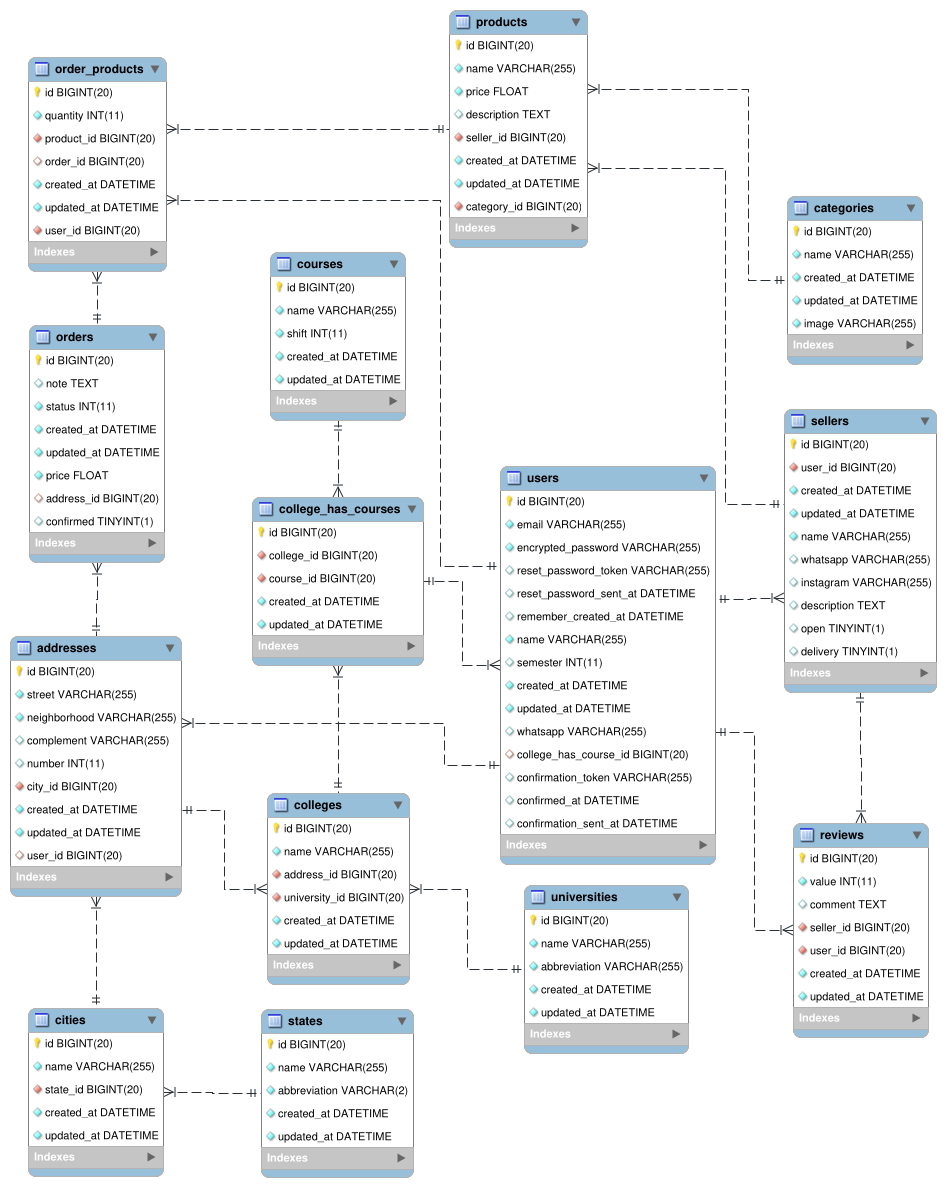
\includegraphics[width=1\textwidth]{figs/err.png}
    \legend{Fonte: Elaborada pelo autor.}
    \label{fig:err}
\end{figure}

\subsection{Telas de \textit{mockup}}\label{mockup}
Foi necessário prototipar a aplicação antes do desenvolvimento, pois com essa abordagem ficou mais fácil e objetivo o desenvolvimento do sistema. Para confecção de cada tela de \textit{mockup}, foi-se utilizada a ferramenta Figma.

O Figma é uma ferramenta de design de interface. Um dos motivos para usar essa ferramenta no projeto foi devido a mesma possuir uma portabilidade muito boa, visto que roda diretamente no navegador, ou seja, é compatível com Windows, Linux e Mac. É multitarefas, ou seja, uma equipe pode explorar o mesmo projeto juntas e ver as alterações em tempo real.

A elaboração dessa etapa foi de suma importância para o resultado final do projeto. Então, para um melhor aproveitamento do dados produzidos, na seção de resultados(XXX) será realizada uma comparação entre as telas de \textit{mockup} e o resultado final da aplicação.

\subsection{Diagrama de casos de uso}
O diagrama de casos de uso é de grande importância para um entendimento geral do sistema, apresentando as principais ações que cada usuário pode fazer. Esse diagrama é apresentado na figura \ref{fig:use}. O cliente pode realizar basicamente três ações. Já pelo vendedor é capaz de realizar outras duas ações além das permitidas quando o mesmo se encontra no papel de cliente do sistema. Em todos os casos é necessário que seja realizado o login na aplicação.
\begin{figure}[htbp!]
  \centering
  \caption{Diagrama de caso de uso}
  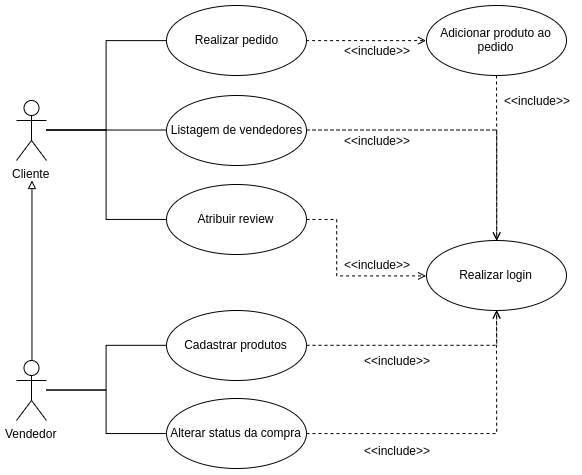
\includegraphics[width=1\textwidth]{figs/caso_de_uso.png}
    \legend{Fonte: Elaborada pelo autor.}
    \label{fig:use}
\end{figure}


\subsection{Diagrama de sequência}
Por meio dos diagramas de sequência será possível ter uma boa visão em relação a cada passo para concluir determinada ação. Nessa seção será apresentado alguns diagramas de sequência que cobrem a todas as funcionalidades do sistema.

\subsubsection{Cadastrar um produto}
Para cadastrar um produto no sistema, será necessário que o usuário tenha perfil tanto de cliente como de vendedor e esteja logado no sistema. Com isso, será possível acessar a área restrita do sistema e solicitar um novo cadastro de produto, inserido cada campo e submetendo para que o registro seja efetuado no banco de dados. Tal diagrama pode ser observado na figura \ref{fig:sequence1}.
\begin{figure}[htbp!]
  \centering
  \caption{Cadastrar um produto}
  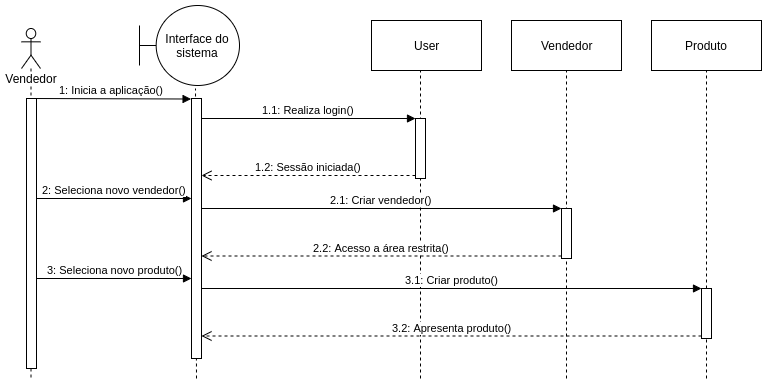
\includegraphics[width=1\textwidth]{figs/sequence1.png}
    \legend{Fonte: Elaborada pelo autor.}
    \label{fig:sequence1}
\end{figure}

\subsubsection{Atribuir um review}
A atribuição de um \textit{review} é uma ação simples, ao qual será necessário que o usuário acesse a página individual do vendedor e clique no link ser redirecionado para a página de inserção do \textit{review}, bastando definir a nota e comentário e submeter ao sistema. Tal diagrama pode ser observado na figura \ref{fig:sequence2}.
\begin{figure}[htbp!]
  \centering
  \caption{Atribuir um review}
  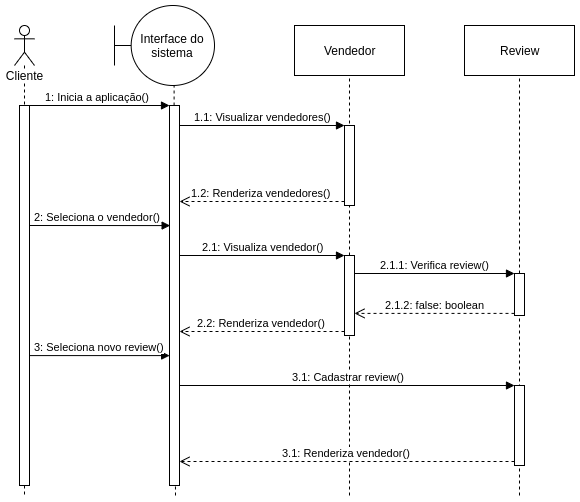
\includegraphics[width=1\textwidth]{figs/sequence2.png}
    \legend{Fonte: Elaborada pelo autor.}
    \label{fig:sequence2}
\end{figure}

\subsubsection{Realizar um pedido}
% escrever aqui
A ação de realizar um pedido é a principal do sistema, ao qual será realizada por um cliente. Será necessário que o cliente insira no carrinho de compras todos os produtos que deseja comprar. Após inserir todos os produtos desejados, deverá acessar a página "minhas compras" e fechar o pedido para que o mesmo seja processado pelo seu vendedor. Tal diagrama pode ser observado na figura \ref{fig:sequence3}.
\begin{figure}[htbp!]
  \centering
  \caption{Realizar um pedido}
  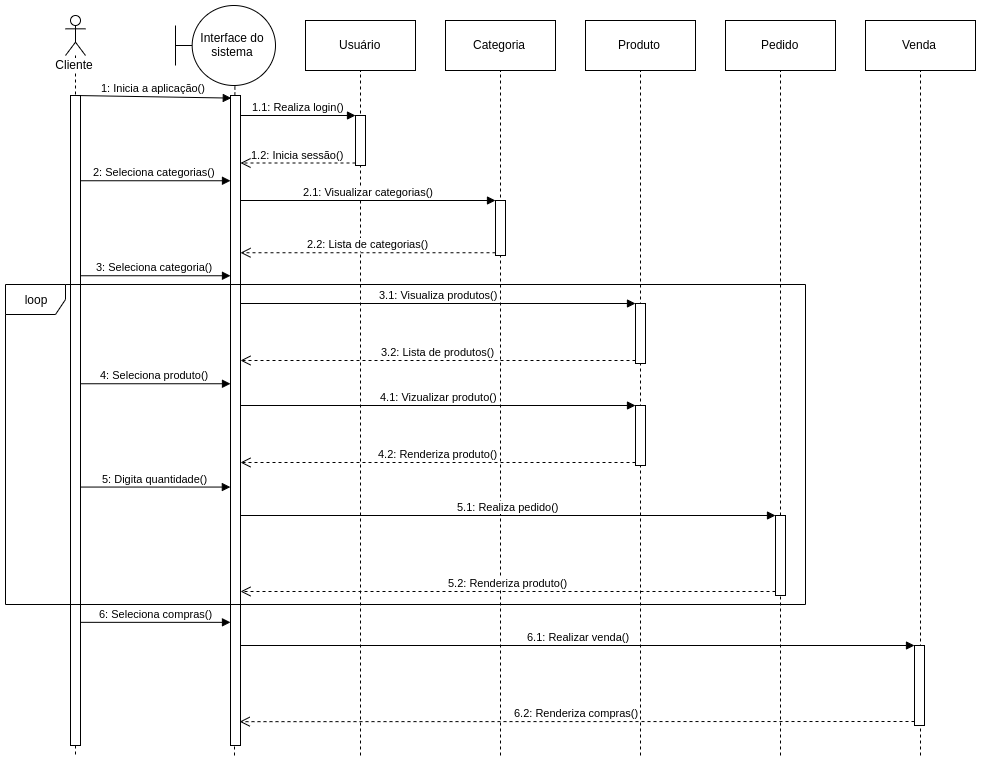
\includegraphics[width=1\textwidth]{figs/sequence3.png}
    \legend{Fonte: Elaborada pelo autor.}
    \label{fig:sequence3}
\end{figure}

\subsection{Diagrama de classes}
A figura \ref{fig:class} representa o diagrama de classes concebido para a aplicação. Todas as classes da aplicação serão derivadas da classe ApplicationRecord do \textit{framework} RoR, omitida nesse diagrama por conter inúmeros atributos e métodos genéricos, ficando assim inviável para apresentação.
\begin{figure}[htbp!]
  \centering
  \caption{Diagrama de classes}
  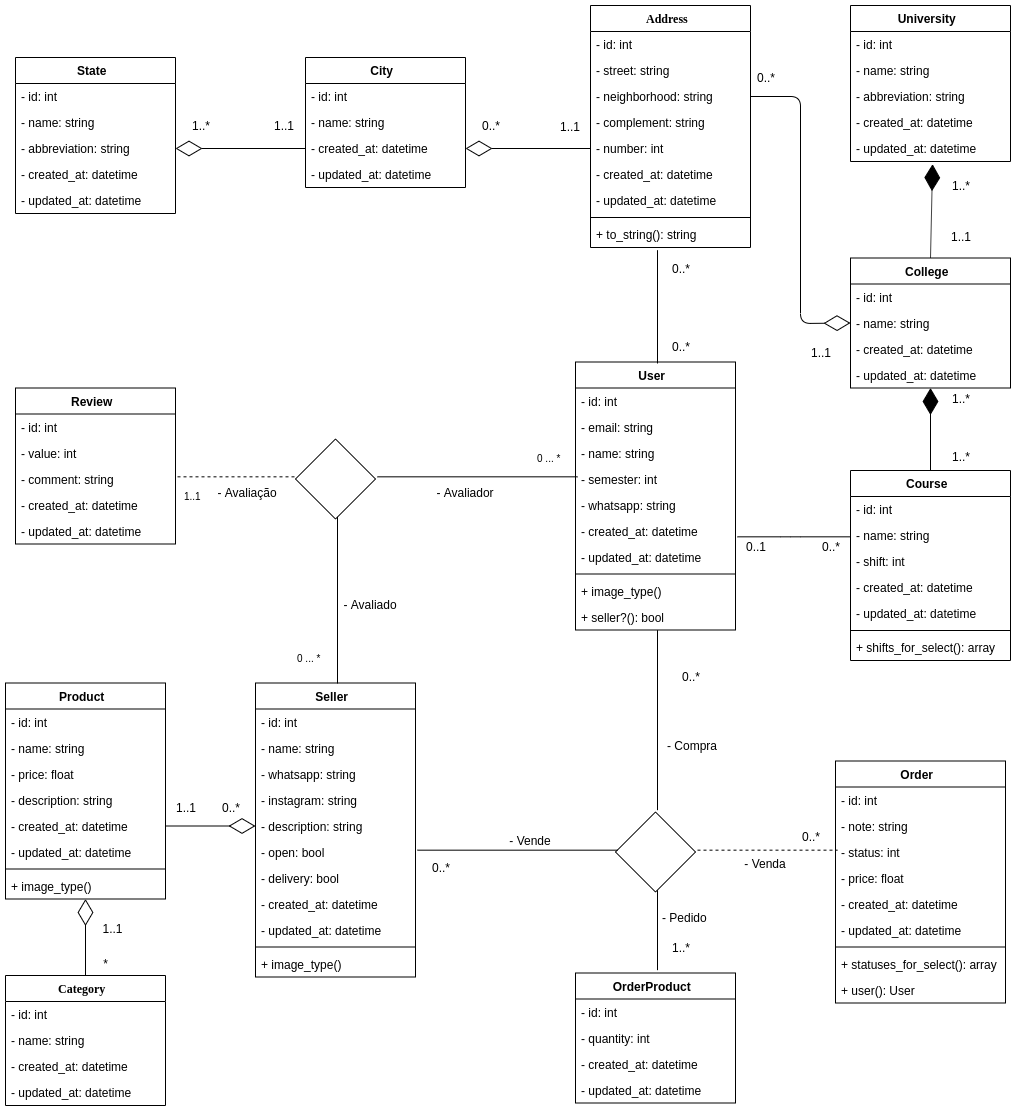
\includegraphics[width=1\textwidth]{figs/class.png}
    \legend{Fonte: Elaborada pelo autor.}
    \label{fig:class}
\end{figure}

\section{Implementação}
O processo de desenvolvimento do sistema utilizou desde o início várias ferramentas auxiliares. Software para versionamento de código, bibliotecas da linguagem, ferramenta de \textit{mockup}(como citada na seção \ref{mockup}) são algumas delas. Tais ferramentas contribuíram agilizar e facilitar o desenvolvimento do projeto.
\subsection{Versionamento de código}
O objetivo mais básico dos softwares de controle de versão é armazenar e gerenciar o histórico de alterações feitas em um arquivo, dessa forma será possível retornar a versões anteriores do seu código caso seja necessário. No projeto aqui desenvolvido foi utilizado o versionador Git. O Git pode se conectar com várias plataformas online, como por exemplo o Github, Gitlab, Bitbucket e outros para que o código fonte seja disponibilizado para o público em geral.
\subsection{Bibliotecas utilizadas}
O RoR também conta vantagem com toda a estrutura das RubyGems da linguagem de programação Ruby, que é um gerenciador de pacotes que fornece um padrão de formato para distribuição de bibliotecas, chamadas de \textit{gem}. Várias \textit{gems} foram utilizadas no atual projeto, muitas delas para facilitar o desenvolvimento, como outras que busca melhorias no código. Na seção \ref{tdd} serão apresentados alguns testes e aplicações das gems no projeto em questão. A seguir será apresentado algumas delas:
\subsubsection{RSpec}\label{rspec}
RSpec é um \textit{framework behaviour-Driven Development}(BDD) de código aberto disponível no Github\footnote{Gem RSpec \url{https://github.com/rspec/rspec}} escrito em Ruby, que permite e facilita a automatização de testes no projeto. Com o RSpec é possível implementar vários tipos de testes, são eles: testes de \textit{model}, testes de \textit{controller} e testes de \textit{view}.
\subsubsection{Rubocop}\label{rubocop}
Rubocop é uma \textit{gem} de código fonte aberto disponível no Github\footnote{Gem Rubocop \url{https://github.com/rubocop-hq/rubocop}} que percorre e verifica se o código segue as boas práticas de programação definidas pelo guia de estilo Ruby. Tal \textit{gem} ajuda a manter os padrões sem que seja preciso conhecer literalmente todas as definições.
\subsubsection{Brakeman}\label{brakeman}
O Brakeman é uma \textit{gem} de código livre disponível no Github \footnote{Gem Brakeman \url{https://github.com/presidentbeef/brakeman}} que ajuda a descobrir várias vulnerabilidades de segurança do projeto. O brakeman roda de forma totalmente automatizada, buscando falhas como \textit{SQL Injection, File Access, Mass Assignment}, dentre outros. Então para ter uma aplicação segura e de qualidade é indispensável o uso dessa \textit{gem}.

\section{Testes automatizados}\label{tdd}
Esta seção avalia de forma sistemática toda a implementação técnica desenvolvida até o momento, busca uma melhor eficiência e qualidade do código da aplicação. Serão realizados quatro tipos de testes automatizados no Mercado Universitário. Testes unitários e integração, testes de segurança e testes de qualidade do código, tais testes serão apresentados a seguir.
\subsection{Testes unitários e integração}
Foi utilizada a gem RSpec para esse tipo de teste. Tal ferramenta foi apresentada na seção \ref{rspec}. De acordo com a imagem \ref{fig:rspec} foram realizados 102 exemplos de testes na aplicação, tais testes conseguiram cobrir 92.9\% de todo o código da aplicação sem que ocorresse nenhuma falha. Tal resultado se mostra bastante satisfatório, uma vez que se aproxima bastante de 100\% de cobertura do código e não apresenta nenhuma falha.
\begin{figure}[htbp!]
  \centering
  \caption{Saída do terminal para teste automatizado unitário e de integração utilizando a \textit{gem} RSpec}
  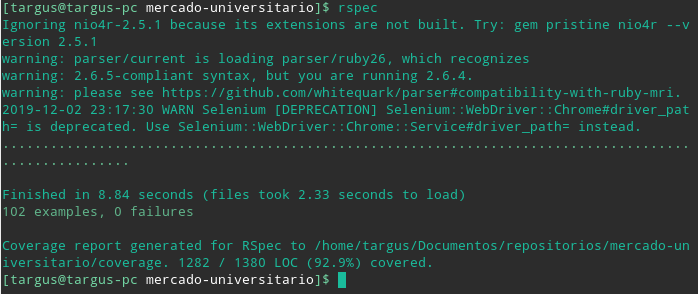
\includegraphics[width=1\textwidth]{figs/rspec.png}
    \legend{Fonte: Elaborada pelo autor.}
    \label{fig:rspec}
\end{figure}
\subsection{Testes de segurança}
Foram utilizadas duas \textit{gems} para realizar esse teste de grande importância para a aplicação. A \textit{gem} Brakeman em conjunto com a \textit{gem} Bundle Audit são suficientes para explorar as principais vulnerabilidades das aplicações web. Como é observado nas imagens \ref{fig:brakeman} e \ref{fig:audit}, não foram encontradas nenhuma vulnerabilidade na aplicação.
\begin{figure}[htbp!]
  \centering
  \caption{Saída do terminal para teste automatizado de segurança utilizando a \textit{gem} Brakeman}
  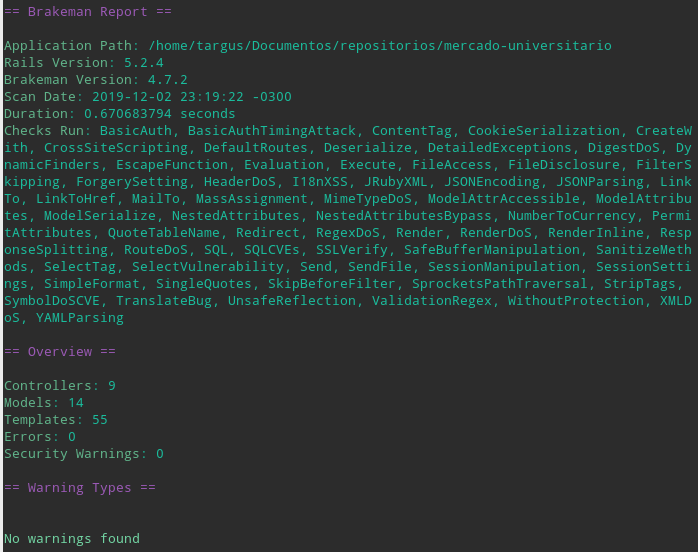
\includegraphics[width=1\textwidth]{figs/brakeman.png}
    \legend{Fonte: Elaborada pelo autor.}
    \label{fig:brakeman}
\end{figure}
\begin{figure}[htbp!]
  \centering
  \caption{Saída do terminal para teste automatizado de segurança utilizando a \textit{gem} Bundle Audit}
  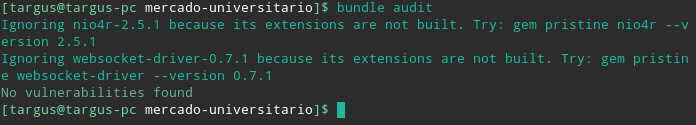
\includegraphics[width=1\textwidth]{figs/bundle_audit.png}
    \legend{Fonte: Elaborada pelo autor.}
    \label{fig:audit}
\end{figure}
\subsection{Testes de qualidade do código}
Para ser possível garantir uma boa manutenção e legibilidade futura do código, foi necessário utilizar a \textit{gem} Rubocop(apresentada na seção \ref{rubocop}). Como observado na imagem \ref{fig:rubocop}, foram verificadas as boas práticas de programação determinadas pelo Rails em 71 arquivos do projeto, não foi encontrada nenhuma ofensa no código.
\begin{figure}[htbp!]
  \centering
  \caption{Saída do terminal para verificação da qualidade do código utilizando a gem Rubocop}
  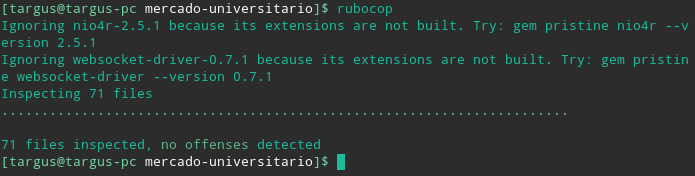
\includegraphics[width=1\textwidth]{figs/rubocop.png}
    \legend{Fonte: Elaborada pelo autor.}
    \label{fig:rubocop}
\end{figure}